\textbf{Finding.} The final modulus products are a small part of the cost. Both methods spend substantial time constructing radial responses and synthesizing angular fields. DSpec's tested tensor prototype moves much of its angular arithmetic into BLAS, but still pays for coefficient packing, copied BLAS buffers, map-based grid addressing, rotations and output movement. YSpec uses direct degree-contiguous angular sums and an ODE boundary-response method. Its fine phase timers are more intrusive, so native totals and instrumented components are reported separately.
\section{Native comparison and experiment}
\begin{center}\begin{tabular}{rrrrrr}\toprule
$L$ & bins & objectives & DSpec (ms) & YSpec (ms) & DSpec/YSpec\\\midrule
3 & 3 & 1 & 38.80 & 32.04 & 1.211\\
6 & 3 & 1 & 155.14 & 160.92 & 0.964\\
12 & 3 & 1 & 239.72 & 251.94 & 0.951\\
12 & 3 & 2 & 323.39 & 320.65 & 1.009\\
12 & 12 & 1 & 853.86 & 1,153.28 & 0.740\\
12 & 48 & 1 & 3,244.47 & 6,554.70 & 0.495\\
\bottomrule\end{tabular}\end{center}
Each native entry is the median of three fresh processes, one numerical thread on one fixed allowed CPU, alternating solver/build order. These are complete numerical API times, including first-use plans and return cleanup, excluding frontend input/setup and export. DSpec sums its objective calls; YSpec handles objectives in one batch. Volume-only comparisons disable source contacts. A separate contact-enabled DSpec case follows.

The homogeneous shell fixture uses full gravity, no attenuation, SEM order parameter NN=8, the original 50 km-deep source and 3 km-deep receiver, and 56 one-sided element/radius traces. $L=3$ has 192 angles (10,752 points); $L=6,12$ have 1,352 angles (75,712 points). The selected direct tensor route retains the original arbitrary-radius compatibility grid; this is not a test of making native SEM output the default. Maximum frequencies for 3, 12 and 48 bins are respectively 1.171875, 4.6875 and 18.75 mHz.\footnote{Bins are $k/(128\times20\,\mathrm{s})$, $k=1,\ldots,F$, with damping $1/360\,\mathrm{s}^{-1}$. A bounded degree/frequency fixture is not a convergence result for a full Earth calculation.}

DSpec additionally returns raw/processed receiver spectra and the objective. YSpec's sampled API returns volume kernels and computes eight elastic/Q channels; only the five common elastic moduli are exported. These differing products are costed explicitly, rather than hidden behind an equal-work claim.

\clearpage\section{What the mathematics asks each solver to do}
For each active frequency and spherical-harmonic family, DSpec forms
\begin{equation}
H_\ell(z)=K_\ell-z^2M_\ell,\qquad
H_\ell u_\ell=b_\ell,\qquad
H_\ell^{H}\lambda_\ell=R_\ell^{H}\widehat q,
\quad \widehat q=\mathcal P^*q.
\end{equation}
The prototype shares one equilibrated sparse LU factorization between forward and Hermitian-adjoint substitutions. ``One forward and one adjoint field'' does not mean two scalar solver calls: at $L=12$ each bin has 12 spheroidal, 12 toroidal and one radial operators, hence 75 distinct dynamic matrices over three bins. The measured one-objective route factors each once.

YSpec instead integrates radial ODE response systems,
\begin{equation}
\frac{dy}{dr}=A_\ell(r,z)y,
\end{equation}
constructing upward/downward boundary solutions, determinant and source-jump matching, spheroidal $b$-vector transport, and physical radial responses at requested nodes. Forward source and receiver unit-force responses share these fundamentals. It has no SEM matrix assembly or LU stage to time.

Both methods reconstruct six spin-strain components using radial coefficients:
\begin{equation}
\varepsilon_s(r,\Omega;z)=
\sum_{\ell,m} c_{s\ell m}(r,z)\,
 d^\ell_{s m}(\theta')e^{im\phi'},\qquad s=0,0,1,-1,2,-2.
\end{equation}
The tensor prototype evaluates these sums as $E=BC$ across 16-radius tiles, then rotates and scatters to output points. Angular geometry and basis values are frequency-independent and reused. YSpec builds tables in 64-angle blocks at each frequency, reusing each table over every radial node; its degree dots use complex coefficients and real Legendre values.

Finally, both form local bilinear elastic energy products and sum their correctly weighted real parts over frequency:
\begin{equation}
K_p(r,\Omega)=\sum_k w_k\,\Re\,B_p
\bigl(\varepsilon^F_k,\varepsilon^A_k\bigr).
\end{equation}
The dual/conjugation convention is carried by each implementation's coefficients. Summing each field over frequency before multiplication introduces unwanted cross-frequency products. Exact covariance contractions can reorder the frequency sum of coefficient \emph{products}; that alternative was explored in the previous audit and is not the direct tensor route profiled here.

The one-objective DSpec path still solves the full weighted global adjoint RHS plus a supplemental minimal receiver basis, even with contacts disabled. The two-objective cache path uses only the minimal unit-force basis and mixes weighted adjoints algebraically. Their different first-call costs must not be attributed solely to cache hits.

\clearpage\section{DSpec: complete three-bin component accounting}
At $L=12$, one objective, native median is 239.72 ms. The representative instrumented run totals 242.20 ms. Entries below are disjoint exclusive times; their unrounded sum closes the API root.
\begin{center}\small
\begin{tabular}{p{.72\textwidth}rr}\toprule Component & ms & \%\\\midrule
Measurement adjoint $\mathcal P^*$ & 0.60 & 0.25\\
Dynamic $H_\ell(z)$ assembly & 8.59 & 3.55\\
Matrix equilibration and scaling & 5.30 & 2.19\\
Sparse symbolic analysis & 5.75 & 2.37\\
Sparse numerical factorization & 28.18 & 11.63\\
Factor dispatch and wrapper overhead & 0.11 & 0.05\\
Forward substitutions, including scaling & 6.20 & 2.56\\
Hermitian-adjoint substitutions, including scaling & 24.75 & 10.22\\
Source lifts, receiver QR, modal recovery & 16.96 & 7.00\\
Radial interpolation and strain numerators & 7.20 & 2.97\\
Representative/receiver sampling and record capture & 2.81 & 1.16\\
Full-volume semantic key construction/lookup & 2.60 & 1.07\\
Cold tensor grid layout and maps & 8.31 & 3.43\\
Angular geometry, Wigner tables and basis plans & 14.07 & 5.81\\
Volume result allocation and material tagging & 13.31 & 5.50\\
Actual complex BLAS matrix products & 20.86 & 8.61\\
BLAS layout conversion, buffers and copies & 16.10 & 6.65\\
Radial coefficient keys, packing and tile scatter & 15.93 & 6.58\\
Volume spin rotations and scatter & 23.40 & 9.66\\
Degree-zero scatter & 4.64 & 1.92\\
Forward-field cache lookup, store and copy & 0.00 & 0.00\\
Receiver spectra scatter & 0.00 & 0.00\\
Pointwise modulus products and scatter & 2.93 & 1.21\\
Contact branch (disabled in main comparison) & 0.00 & 0.00\\
Forward processing $\mathcal P$, FFT/window & 0.10 & 0.04\\
Final objective inner product & 0.00 & 0.00\\
Tensor bookkeeping, allocation and cleanup remainder & 7.84 & 3.24\\
API bookkeeping, copies and cleanup remainder & 5.67 & 2.34\\
\midrule Total instrumented API & 242.20 & 100.00\\\bottomrule\end{tabular}\end{center}
Nested solve scopes provide a useful further split without being added again: full weighted adjoint solves and minimal supplemental basis solves are shown in the machine-readable stage table. Radial strain time includes interpolation-plan use and strain-numerator construction; it is not a pure interpolation-only timer. No interpolated raw-strain approximation is introduced.
\clearpage\section{YSpec: complete three-bin component accounting}
At $L=12$, one objective, native median is 251.94 ms. The representative instrumented run totals 302.54 ms. These are instrumented durations, not a synthetic rescaling of native time.
\begin{center}\small
\begin{tabular}{p{.72\textwidth}rr}\toprule Component & ms & \%\\\midrule
API geometry, sampling and measurement setup & 0.35 & 0.12\\
Measurement/basis frequency weights & 0.00 & 0.00\\
Initial conditions and upward ODE integration & 50.20 & 16.59\\
Initial conditions and downward ODE integration & 0.40 & 0.13\\
Spheroidal source-jump $b$-vector transport & 39.79 & 13.15\\
Determinants, jumps, matching and transport & 3.99 & 1.32\\
Physical radial variable recovery & 0.47 & 0.15\\
Combine source/receiver coefficients and strains & 0.82 & 0.27\\
Radial context and family driver overhead & 0.28 & 0.09\\
Forward source and receiver unit-force weights & 0.03 & 0.01\\
Wigner and generalized-Legendre tables & 12.53 & 4.14\\
Source angular harmonic sums & 81.94 & 27.08\\
Adjoint angular harmonic sums & 51.52 & 17.03\\
Relative-frame spin rotations & 12.96 & 4.28\\
Five-modulus strain-energy pair products & 6.64 & 2.19\\
Objective mixing and eight parameter products & 8.08 & 2.67\\
Frequency/dispersion parameter weights & 0.00 & 0.00\\
Block-to-output frequency accumulation & 1.98 & 0.66\\
Output transforms, scaling and construction & 5.46 & 1.81\\
Angular-block allocation, loop and cleanup remainder & 23.20 & 7.67\\
API allocation, bookkeeping and cleanup remainder & 1.90 & 0.63\\
\midrule Total instrumented API & 302.54 & 100.00\\\bottomrule\end{tabular}\end{center}
The energy-pair row computes the five bilinear modulus terms. The parameter-products row includes measurement/basis mixing and eight output channels, including three Q channels even for this non-attenuating calculation. It therefore covers more than five final multiplications. The angular-block remainder includes allocation, loop control, temporary energy-vector handling, cleanup and timer boundary overhead; it is retained explicitly.
\clearpage\section{Why the wider frequency band separates the methods}
\begin{center}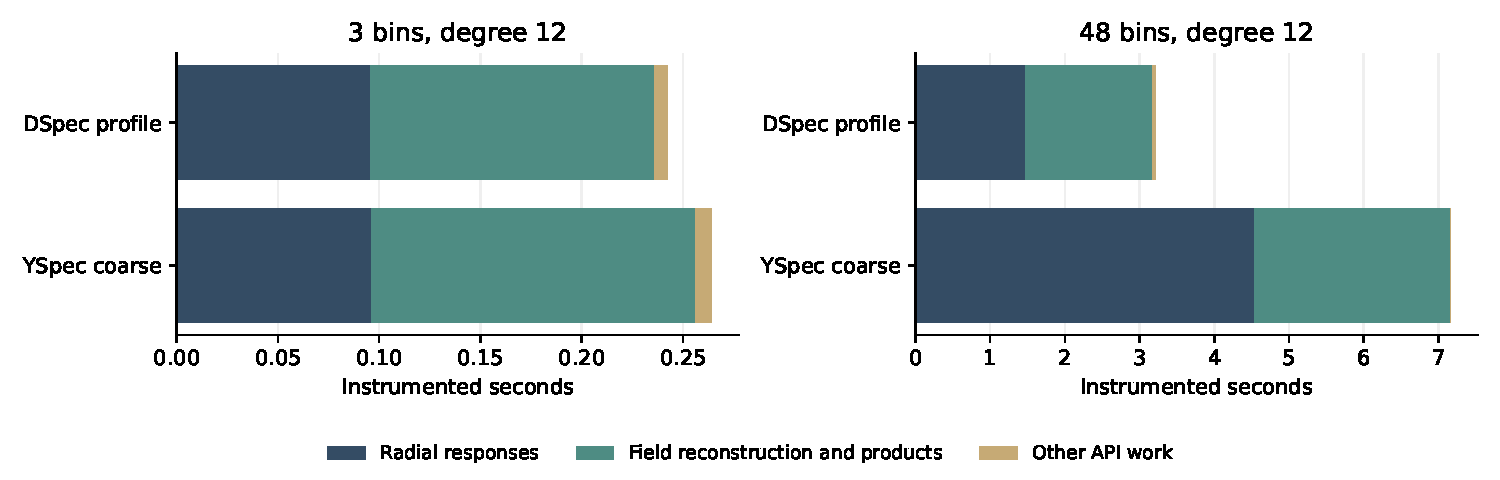
\includegraphics[width=\textwidth]{stage-partitions.pdf}\end{center}
\noindent\small The bars partition instrumented API roots exactly. DSpec's field block includes radial strain evaluation and the final point-kernel pass; YSpec forms radial strain coefficients in the radial block and fuses angular sums with products. These are comparable pipeline regions, not identical kernels. YSpec's coarse build has no per-point phase clocks or fine-child commits.\normalsize
\begin{center}\small\begin{tabular}{p{.68\textwidth}rr}\toprule
Measured work & 3 bins (ms) & 48 bins (ms)\\\midrule
DSpec numerical LU & 28.18 & 431.75\\
DSpec forward + adjoint substitutions & 30.95 & 496.08\\
DSpec actual complex GEMM & 20.86 & 323.77\\
DSpec coefficient packing + BLAS buffers & 32.03 & 477.85\\
DSpec volume rotations/scatter & 23.40 & 362.35\\
DSpec final modulus products & 2.93 & 49.92\\
YSpec up/down ODE integration (coarse) & 51.18 & 2,528.86\\
YSpec source $b$ transport (coarse) & 39.65 & 1,913.07\\
YSpec whole angular/product block (coarse) & 159.76 & 2,614.12\\
\bottomrule\end{tabular}\end{center}
YSpec attempts 78,751 Runge--Kutta steps and evaluates 481,137 RHS callbacks over three bins. At 48 bins these rise to 3,998,468 and 24,129,174: about 51 and 50 times the work for 16 times as many bins. Its higher-frequency ODE integration/transport cost explains much of the growing gap. DSpec factors 75 versus 1,200 operators of the same bounded SEM sizes.

Actual DSpec complex-GEMM terms are 125,473,464 versus 2,007,575,424; YSpec performs 141,732,864 versus 2,267,725,824 complex-coefficient/real-Legendre degree terms. These are different operation types, not equal FLOP counts. Counting only $75{,}712\times6$ output strain slots misses the degree/order sums, two fields and frequency loop.

\clearpage\section{Repeated objectives, source contacts and frontend costs}
At $L=12$, three bins, DSpec's two-objective native total is 323.39 ms, against YSpec's 320.65 ms. DSpec's native median call durations are 234.24 and 89.28 ms. Their individual medians need not sum to the median of process totals.

The representative instrumented DSpec calls take 241.05 and 92.87 ms. The first factors all 75 operators; the second factors none, hits 75 radial-response entries and all three forward angular-field entries. It still performs weighted-adjoint reconstruction, source/modal bookkeeping, representative radial coefficient sampling, adjoint angular synthesis, point products and result allocation. Full-source angular synthesis and receiver-suffix sampling are skipped on the cache hit; workspace preparation and coefficient gathering are not.

The one-objective nonbatch path solves 219 forward RHS columns, 1,011 full weighted global-adjoint columns and 108 supplemental unit-basis columns. The two-objective batch path actually solves 219 forward plus 111 unit-basis columns once, then reconstructs the 2,022 requested weighted columns across both calls. Submitted cache RHS widths are not counts of substitutions on cache hits.

YSpec's two-objective batch retains the same 75 ODE response-family solves and the same 481,137 RHS evaluations. A second independent receiver direction adds coefficient combinations and angular/bilinear work rather than another fundamental radial integration. These are two different ways of sharing response information.

\textbf{Source contacts.} In a separate, nonbatch, contact-enabled DSpec run, the contact branch costs 2.38 ms across three bins. Native total is 239.12 ms; the small difference from the contacts-off total is within the observed run spread, so subtracting the totals is not a valid contact timer. All six contact-enabled clone/output comparisons pass with zero contact error. YSpec's sampled API omits this source-shell term; no contact speed ratio is claimed.

\begin{center}\small\begin{tabular}{p{.68\textwidth}rr}\toprule
Three-bin boundary & DSpec (ms) & YSpec (ms)\\\midrule
Frontend setup, native median & 53.52 & 42.29\\
Model/input to returned arrays, native median & 295.65 & 298.45\\
Export, native median (binary versus CSV) & 11.18 & 369.27\\
\bottomrule\end{tabular}\end{center}
DSpec's representative setup includes 48.49 ms sample-CSV parsing, 1.74 ms SEM construction and 3.93 ms stream/coordinate export. YSpec frontend setup combines model/configuration/sample preparation. Output formats differ; their export times are not solver times.

The DSpec diagnostic executable also runs a separate reference calculation after every candidate call: native medians are 643.56 ms (three bins) and 10,032.04 ms (48 bins), plus roughly 3 ms validation and 11 ms binary export. This harness verification is excluded from solution-only API and model-to-array times. The benchmark wrapper's wall time additionally includes parent-side hashing/compression/comparison and must not be presented as child solver time.

\clearpage\section{Calibration, completeness and validation}
\begin{center}\small\begin{tabular}{lrrr}\toprule
$L$/bins/objectives & DSpec profile (\%) & YSpec coarse (\%) & YSpec fine (\%)\\\midrule
3/3/1 & -3.0 & -4.8 & +17.4\\
6/3/1 & -2.7 & +3.1 & +28.2\\
12/3/1 & +1.0 & +4.9 & +20.1\\
12/3/2 & +3.3 & +3.7 & +19.1\\
12/12/1 & +0.1 & +5.3 & +15.6\\
12/48/1 & -1.1 & +9.3 & +14.1\\
\bottomrule\end{tabular}\end{center}
Percentages compare instrumented median API time with the separate native median. They include hook perturbation and run-to-run variability; negative values do not mean instrumentation accelerates the solver. At the main $L=12$/three-bin point, native ranges are 238.82--246.66 ms for DSpec and 251.07--266.61 ms for YSpec.

YSpec fine timing accumulates raw phase intervals inside its original fused node/place/basis loop, with no new angular work buffers or changed operation order. It makes 2,725,632 fine timer reads at three bins, so small phase durations include appreciable timer boundary cost. Coarse timing compiles those phase hooks and child commits out while retaining outer scopes and counters. The difference is combined fine-hook perturbation, not a pure clock latency measurement. Its legacy \texttt{angular\_phase\_timer\_reads} counter counts disabled call sites, not actual clock reads. Neither detailed table should be relabeled as exact native per-component time, and no global rescaling is used.

All API components, including retained bookkeeping/cleanup remainders, are assigned once by exclusive time. For every root,
\begin{equation}
t_{\mathrm{API}}=\sum_s t_s^{\mathrm{exclusive}}.
\end{equation}
Closure errors are zero to floating-point summation roundoff (maximum below $10^{-8}$ s). Representative tables use the process with median instrumented API duration, so their unrounded rows close their own root; they are not sums of independently chosen component medians. Rounded table rows may differ in the last printed digit.

The final matrix comprises 84 processes, plus 18 coarse-control and seven contact processes: 109 final processes. All 96 clone-versus-original output gates pass; arrays are byte-identical in all these comparisons. DSpec also retains its original per-process reference comparison. Setup and export have independent accounting roots. Diagnostic packet export is disabled. No timings overlap compilation or another campaign numerical run; each process is pinned to one fixed allowed CPU with one numerical thread, a 180 s CPU limit and 3 GiB address-space limit. Hardware performance counters were unavailable, so these are wall-time scopes and exact software work counters, not PMU measurements.\footnote{Portable GCC Release/O3 without fast-math; original equilibrated DSpec solver and cached YSpec dependency library retained. Process address-space limits are not an aggregate kernel-enforced campaign memory budget.}

Frozen source review restored YSpec's original early-exit scan and DSpec's direct initialization forms before final runs. All 366 production DSpec tracked-file hashes and seven Phase0 artifact hashes are unchanged; its existing dirty state is preserved. YSpec remains clean at \texttt{280eab0}; DSpec remains at \texttt{a778b13}. All 14 protected original prototype files and 66 profiling source/build/runtime files verify against pre-run hashes. Instrumentation equivalence inherits the prototype's previous scientific checks; it adds no convergence claim or new whole-planet receiver accuracy claim.

\clearpage\section{What the profile says to improve next}
\begin{enumerate}
\item \textbf{Remove avoidable data preparation in the direct tensor path.} Canonical coefficient indices and retained BLAS-ready bases can eliminate repeated map construction, tile reordering and basis copies. Current packing plus BLAS buffers cost 32.03 ms at three bins and 477.85 ms at 48 bins, versus 20.86 and 323.77 ms in actual matrix-product scopes. These are measured costs to target, not guaranteed removable savings.
\item \textbf{Make the volume-only minimal-adjoint path explicit.} The current one-objective branch computes both the full weighted global adjoint and a supplemental receiver basis. The nested full-weighted solve scope alone costs 21.28 ms at three bins. The batch route already demonstrates basis reuse, but source contacts require their separate validated path and cache failure/admission rules still need integration work. Reusing symbolic sparsity analysis is another smaller target; numerical factors still change with frequency.
\item \textbf{Fuse field movement, relative rotation and energy products.} Volume rotations/scatter cost 23.40 ms, result allocation/tagging 13.31 ms, and separate degree-zero scatter 4.64 ms at three bins. YSpec shows the alternative common-frame fused product organization. Validate spin/dual signs, TI invariance, fluid behavior and source-contact separation before integrating this change.
\item \textbf{Fix reuse admission and grid addressing before chasing tiny products.} At 48 bins DSpec builds two tensor frame plans but records 104 basis misses, compared with 14 at three bins. Retained plan payload reaches 33,528,992 bytes of a 33,554,432-byte admission budget. The counters are consistent with two bases being rebuilt at each additional frequency because the remaining payload cannot admit them. Compact grid addressing and avoiding duplicated basis/storage payload should be evaluated before increasing the budget. The cold grid map is 8.31 ms; repeated full-volume semantic keys cost 38.79 ms across 48 bins.
\item \textbf{Keep covariance and native SEM output as separate decisions.} Exact frequency covariance could remove repeated field synthesis and some buffers, but the current BLAS arithmetic is already fast and radial work remains substantial. A useful integrated covariance implementation must eliminate packing/movement as well as contractions. Native SEM output is a useful representation feature; the previous audit's strict high-degree native-node discrepancy must be resolved before adopting it as the default. Radial interpolation/strain construction here is only 7.20 ms, so it does not explain the present runtime.
\end{enumerate}
These are proposed follow-on changes. This profiling follow-up changes only isolated instrumentation; it does not promote a new numerical route to production.

\section{Evidence and reproducibility}
The follow-up evidence root is \texttt{math-profile/}, beside the previous \texttt{algorithm-audit/} under this chat's \texttt{investigations/dspec-sk-profile-20261026/}. The report tables and vector plot are generated directly from \texttt{summary.json}. Exact native ranges, medians, selected run indices, every stage/counter and every gate remain in the saved JSON.
\begin{center}\small\begin{tabular}{p{.45\textwidth}p{.49\textwidth}}\toprule
Evidence & Location relative to the follow-up root\\\midrule
All 2,781 component timings & \texttt{all-stage-times.csv}\\
Exhaustive 105-stage mathematical map & \texttt{complete-component-map.json}\\
Native/fine full matrix and arrays & \texttt{runs-01/}\\
No-fine-hook YSpec control & \texttt{coarse-runs-01/}\\
Separate source-contact case & \texttt{contacts-01/}\\
Exact configuration/resource protocol & \texttt{protocol.json}\\
Instrumented source/build freeze & \texttt{final-before-runs.sha256.json}\\
Production/prototype preservation & \texttt{preservation-verification.json}\\
Fresh independent reviews & \texttt{review/}\\
\bottomrule\end{tabular}\end{center}

